\documentclass[print]{tudelft-report}

\usepackage{hyperref}
\usepackage{graphicx}
\usepackage{placeins}
\usepackage{amsmath}
\usepackage{longtable}
\usepackage[acronym]{glossaries}
\usepackage[backend=bibtex]{biblatex}
\usepackage[labelfont=bf]{caption}
\usepackage{cleveref}
\usepackage{glossary-superragged}
\usepackage{afterpage}
\usepackage[toc,page]{appendix}

\DeclareNameAlias{sortname}{last-first}
\DeclareNameAlias{default}{last-first}

\setacronymstyle{short-long}
\makeglossaries
\loadglsentries{acronyms}
\renewcommand{\glsnamefont}[1]{\textbf{#1}}

\addbibresource{report22.bib}

\hypersetup{
    colorlinks,
    citecolor=cyan
}

\begin{document}
%% Use Roman numerals for the page numbers of the title pages and table of
%% contents.
\frontmatter

\cleardoublepage
\title[MSc Thesis Report]{Perturbed orbital motion of \\ regolith around Asteroids}
\author{Abhishek Agrawal}
\affiliation{Delft University of Technology}
\coverimage{backgroundimg_asteroid_2.jpg}
\makecover

%% Include an optional title page.
%\begin{titlepage}


\begin{center}

%% Insert the TU Delft logo at the bottom of the page.

%% Print the title in cyan.
{\makeatletter
% \titlestyle\fontsize{64}{94}\selectfont\@title
\titlestyle
\color{tudelft-cyan}
\fontsize{34}{30}
\selectfont{Orbital motion of regolith around asteroids \par}
%\titlestyle\color{tudelft-cyan}\Huge\@title
% \titlestyle\color{tudelft-cyan}\Huge{Perturbed orbital motion of regolith around asteroids}
\makeatother}

\bigskip
\bigskip
%% Print the optional subtitle in black.
{\makeatletter
\ifx\@subtitle\undefined\else
    \bigskip
   {\tudsffamily\fontsize{16}{32}\selectfont\@subtitle}
    %\titlefont\titleshape\LARGE\@subtitle
\fi
\makeatother}

\bigskip
\bigskip

by
%door

\bigskip
\bigskip

%% Print the name of the author.
{\makeatletter
%\largetitlefont\Large\bfseries\@author
\titlestyle\fontsize{26}{26}\selectfont\@author
\makeatother}

\bigskip
\bigskip

to obtain the degree of Master of Science in Aerospace Engineering
%ter verkrijging van de graad van Master of Science

at Delft University of Technology
%aan de Technische Universiteit Delft,

% defended publicly on Wednesday March 27, 2018
\bigskip\bigskip
Tuesday March 27, 2018
%in het openbaar de verdedigen op dinsdag 1 januari om 10:00 uur.

\vfill

\begin{tabular}{lll}
    Student number: & 4416600 \\
    % Project duration: & \multicolumn{2}{l}{September 1, 2016 -- January 1, 2013} \\
    Thesis committee: & Prof. Dr.\ Ir.\ D.J.\ Scheeres & University of Colorado, Boulder, supervisor \\
        & Ir.\ R.\ Noomen & TU Delft, supervisor \\
        & Prof. Dr.\ Ir.\ P.N.A.M. Visser\ & TU Delft, chair \\
        & Dr.\ Angelo Cervone\ & TU Delft, external
\end{tabular}
%% Only include the following lines if confidentiality is applicable.

\bigskip
\bigskip
% \emph{This thesis is confidential and cannot be made public until January 31, 2018.}
%\emph{Op dit verslag is geheimhouding van toepassing tot en met 31 december 2013.}

\bigskip
\bigskip
An electronic version of this thesis is available at \url{http://repository.tudelft.nl/}.
%\\[1cm]

%\centering{\includegraphics{cover/logo_black}}


\end{center}

\begin{tikzpicture}[remember picture, overlay]
    \node at (current page.south)[anchor=south,inner sep=40pt]{
        \centering{
\includegraphics{cover/combined_logo_black}}
    };
\end{tikzpicture}

\end{titlepage}


%For image credit on page behind title page.
\thispagestyle{empty}
\placetextbox{0.500}{0.07}{Cover image credit: Adopted from European Southern Observatory. Artist's Impression of the binary asteroid Antiope.}%
\cleardoublepage

%Fancy quote
\dedication{
\begin{center}
\textit{"If you wish to make an apple pie from scratch, you must first invent the universe."}%

Carl Sagan
\end{center}}

\chapter*{Preface}
\setheader{Preface}
\addcontentsline{toc}{section}{Preface}
% After 45 years since the day man landed on the Moon, mankind created history, yet again. For the first time ever, a spacecraft was put into an orbit around a comet and a lander was deployed to its surface. This was the Rosetta mission; launched in March 2004, the spacecraft took an astonishing 10 years to travel to the comet 67P/Churyumov-Gerasimenko, finally arriving at the comet in August 2014. This is an immense achievement for the scientists and engineers involved in the Rosetta mission because space missions to small irregular bodies in our solar system, both comets and asteroids, pose significant dynamical challenges. For scientists, missions to comets and asteroids are of great interest since in-situ exploration of these small bodies can provide insight into the birth of our Solar System and answer some very important and fundamental questions such as those about the origins of life on Earth. Now even the private space industry is interested in these small bodies, such as in mining the vast reserves of untapped natural resources within the small bodies. For a student, designing and assessing orbits around a small irregular body, and in our case an asteroid, turns out to be one of the toughest problems in astrodynamics, making it a perfect research topic for an MSc Thesis.

% This report serves to be a \textit{Literature Study} in the framework of the Master's program at the Faculty of Aerospace Engineering, Delft University of Technology. It paves way for the upcoming thesis project, where the actual research work shall be carried out. I am grateful I could do this literature study under the supervision of my supervisor Ir. Ron Noomen and with support from Dr. Jinglang Feng. Their experience in the subject matter has been of tremendous help to me. In writing this report, I have tried my very best to ensure that the material in the report is presented in a manner which is pleasant to read and understand. I hope you can gain some valuable knowledge from reading this report.

...[TBD]...

\begin{flushright}
{\makeatletter\itshape
    \@author \\
    Delft, August 2016
\makeatother}
\end{flushright}


\tableofcontents
\chapter*{List of Symbols}
\label{los}
\markboth{List of Symbols}{}
\addcontentsline{toc}{chapter}{List of Symbols}

\subsection*{Latin Letters}
\begin{longtable}[l]{p{100pt} p{70pt} p{250pt}}
\textbf{Symbol} & \textbf{Units} & \textbf{Description}             \\

$r$             & $m$           & position vector magnitude         \\
$\mathbf{r}$    & $m$           & position vector                   \\
$U$             & $m^2/s^2$     & Gravitational potential           \\
\end{longtable}

\subsection*{Greek}
\begin{longtable}[l]{p{100pt} p{70pt} p{250pt}}
\textbf{Symbol} & \textbf{Units} & \textbf{Description}             \\

$\alpha$        & $m$           & Largest semi-major axis of tri-axial ellipsoid shaped asteroid \\
\end{longtable}


\glsaddall
%
% \renewcommand{\glstextformat}[1]{\color{orange} #1}
\printglossary[type=\acronymtype, title=List of Acronyms, style=superragged]
\afterpage{\null\thispagestyle{empty}\addtocounter{page}{-1}\newpage}
%

%% Use Arabic numerals for the page numbers of the chapters.
\mainmatter
\binoppenalty=\maxdimen
\relpenalty=\maxdimen

%\input{Folder_Name/chapter_name.tex}
\chapter{Introduction}
\label{chap:intro}
\graphicspath{{Introduction/Images/}}

At the dawn of the nineteenth century, Italian astronomer Giuseppe Piazzi was engrossed in observing the Taurus constellation to update a star catalog. On January 1 1801, atop the Palermo observatory in Sicily, he observed a light which was not mentioned in the catalog. He followed the strange light for a few more nights, eventually realizing that he had discovered a small planet between Mars and Jupiter. He named the minor planet Ceres and it became the first of its kind to be discovered by humans. Broadly speaking, it became the first asteroid to ever be discovered \parencite{cunningham2016discovery}. Soon after this discovery, three other minor planets were discovered in the gap between Mars and Jupiter. Pallas was discovered in 1802, followed by Juno in 1804, and finally Vesta in 1807. After the discovery of Ceres and Pallas, renowned astronomer William Herschel realized that these are a new species of celestial bodies and proposed to call them asteroids (which in Greek means star-like) instead of minor planets. For nearly 40 years after the discovery of Vesta, no additional discoveries were made. Then once again in the second half of the nineteenth century, astronomers started discovering more and more asteroids until they realized that there is a whole belt of it between Mars and Jupiter \parencite{bottke2002asteroids}.
%
\newline\newline
%
Asteroids are rocky, airless celestial bodies in our Solar System that orbit the Sun and are quite small in size compared to the planets. They can be viewed as remnants of the processes that formed the inner planets of our Solar System \parencite{nasa_asteroids_web}. Asteroids are mostly irregularly shaped with a few exceptions, like Ceres, that have a nearly spherical shape. \Cref{fig:asteroid_shapes} provides a view on the different morphologies of asteroids \parencite{nasa_asteroids_web}. They are typically categorized based on their location in the Solar System. A large number of asteroids are found in the region between Mars and Jupiter and are called as \glspl{MBO}. A relatively smaller number of asteroids, called \glspl{NEA}, have orbits that are very close to and/or crosses the heliocentric orbit of Earth. Asteroids at the $L_4$ and $L_5$ Lagrange points of Jupiter, sharing its orbit around the Sun, are termed as Trojans. Then we have Centaurs, asteroids whose orbit lies between or crosses that of the Giant planets in our Solar System. The fifth and the final category is that of the \glspl{TNO} i.e. asteroids with orbit beyond that of Neptune and reaching as far as the Oort cloud \parencite{planetarySciencePater}. The distribution of asteroids in the inner and outer Solar System is shown in \Cref{fig:asteroid_distribution}.
% Asteroids are rocky, airless celestial bodies in our Solar System that orbit the Sun and are found in quite large numbers. Relative to the planets, these asteroids are very small and are sometimes even referred to as minor planets. They can be viewed as remnants of the processes that formed the planets of the inner Solar System. Asteroids come in different shapes and sizes, and while most are irregularly shaped, a few are found to be nearly spherical. \Cref{fig:asteroid_shapes} provides a view on the different morphologies of asteroids \parencite{nasa_asteroids_web}. They are typically classified based on their location in our Solar System. A large number of asteroids are found in the region between Mars and Jupiter, called the \gls{MAB}, and these asteroids are hence called as the \gl{MBO}}. A rather smaller number of objects whose orbit lies close to that of Earth or crosses the Earth's orbit itself are termed as \gl{NEO}}. Next, sharing Jupiter's orbit around its $L_4$ and $L_5$ Lagrange points are the \texti{Trojan} asteroids, and the ones whose orbit lies between or crosses that of the giant planets (Jupiter, Saturn, Uranus, Neptune) in our Solar System are called the \texti{Centaurs}. The vast majority of small bodies in our Solar System have orbits that extend beyond that of Neptune and are termed as \gls{TNO}}. These are further classified into \gls{CKBO}, objects with low eccentric orbits resonant with Neptune, and \gls{SDO}, objects with highly eccentric and non-resonating orbits. There are small bodies even beyond the \gls{TNO}s and are found in a very distant region called the \texti{Oort Cloud} \parencite{planetarySciencePater}. The distribution of asteroids in the inner and outer Solar system is shown in \Cref{fig:asteroid_distribution}.
%%%
\begin{figure}[htb]
\centering
\captionsetup{justification=centering}
    \begin{minipage}{0.48\columnwidth}
        \subfloat[]{
            \includegraphics[width=\columnwidth, height=0.5\textheight, keepaspectratio=true]{asteroid_size_comparison.jpg}
            \label{fig:vesta_compared_with_other_asteroids}
        }
    \end{minipage}
    \begin{minipage}{0.48\columnwidth}
        \subfloat[]{
            \includegraphics[width=\columnwidth, height=0.25\textheight, keepaspectratio=true]{itokawa.jpg}
            \label{fig:itokawa_image}
        }
        \\[3mm]
        \subfloat[]{
            \includegraphics[width=\columnwidth, height=0.25\textheight, keepaspectratio=true]{Ida_Dactyl.jpg}
            \label{fig:ida_dactyl_image}
        }
    \end{minipage}
\caption{Satellite imagery depicting different morphologies of asteroids. \protect\subref{fig:vesta_compared_with_other_asteroids} Size and shape variations amongst a few known asteroids, \protect\subref{fig:itokawa_image} Asteroid Itokawa with its rocky and rough surface, \protect\subref{fig:ida_dactyl_image} Asteroid Ida with its moon Dactyl orbiting around it \parencite{nasa_asteroids_web}.}
\label{fig:asteroid_shapes}
\end{figure}
\FloatBarrier
%%%
Due to their extremely small sizes, asteroids can not have high internal pressures and temperatures, which means that they could have potentially preserved the early chemistry of our Solar System \parencite{hayabusaTouchdownDynamics}. This makes them a valuable source for us to learn about the history and origin of our Solar System. It is hypothesized that during the early years of Earth's formation, carbon-based molecules and other volatile materials which serve as the basic building-blocks of life, could have been delivered to Earth through asteroid impacts \parencite{jpl_asteroid_web}. Finally, some asteroid types are rich in resources and contain vast supplies of precious metals \parencite{asteroidPreciousMetalSource} and water \parencite{asteroidWaterSource}, which could potentially be mined and used to aid further exploration and colonization of our Solar System \parencite{jpl_asteroid_web}. Thus in light of this, asteroid exploration, both in-situ and ex-situ, has gained significant importance not only among the scientific community but among the private space industry as well, with more and more future missions being planned to these small bodies. The \gls{NEAR} spacecraft launched by the \gls{NASA} in 1996, as part of their Discovery program, became the first spacecraft in history to orbit an asteroid (433 Eros) and eventually land on it. The spacecraft spent almost a year around Eros, providing extended and comprehensive observations of surface morphology, shape, internal structure and physical properties of the asteroid \parencite{nearMission}. The Hayabusa mission (formerly MUSES-C) by the \gls{JAXA} entered into orbit around asteroid Itokawa in 2005 and became the first mission to sample the surface of an asteroid, which was subsequently returned to Earth for analysis in 2010 \parencite{yanoHayabusaTouchdown}. These missions have substantially increased our knowledge about the small bodies in our Solar System.
%
\newline\newline
%
%%%
\begin{figure}[htb]
\centering
\captionsetup{justification=centering}
    \subfloat[]{
        \fbox{
        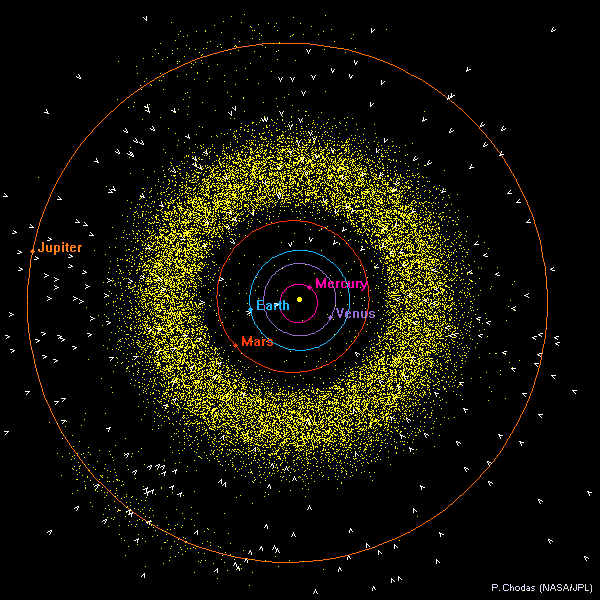
\includegraphics[width=0.5\linewidth, height=\textheight, keepaspectratio=true]{asteroid_distribution_orbit_plot_inverted.png}
        \label{fig:inner_asteroids}
        }
    }
    \subfloat[]{
        \fbox{
        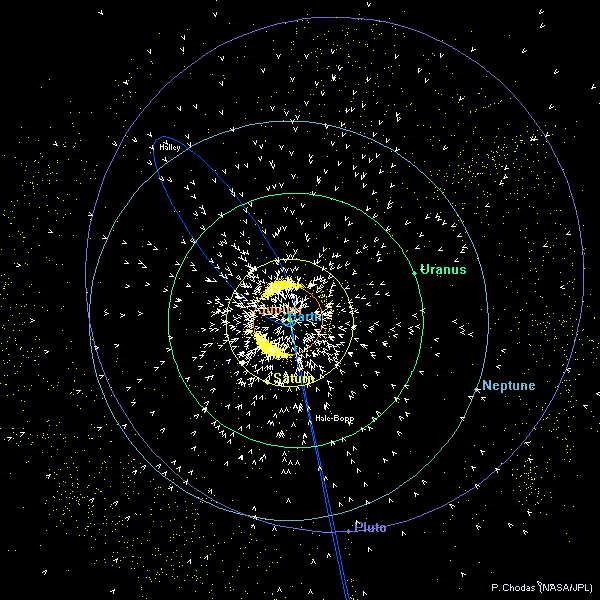
\includegraphics[width=0.5\linewidth, height=\textheight, keepaspectratio=true]{asteroid_distribution_outer_orbit_plot_inverted.png}
        \label{fig:outer_asteroids}
        }
    }
\caption{Distribution of asteroids in \protect\subref{fig:inner_asteroids} inner Solar System and \protect\subref{fig:outer_asteroids} outer Solar System. Asteroid locations are shown by blue-colored dots whereas the black-colored wedges pointing towards the Sun represent the comets. The diagrams are based on the small-bodies cataloged up until November 2016 \parencite{jpl_asteroid_web}. These images are color-inverted versions of the original.}
\label{fig:asteroid_distribution}
\end{figure}
\FloatBarrier
%%%
Two more asteroid rendezvous missions launched quite recently are of particular interest to this thesis. Following the success of Hayabusa, \gls{JAXA} launched another sample return mission called Hayabusa-2 to asteroid 1999 JU3, scheduled to be in orbit around it by mid-2018. It will perform a 1.5 year long close-proximity operation at the asteroid that includes surface sample acquisition, which will eventually be returned to Earth in a capsule, and a \SI{2}{\metre} wide cratering event to observe the sub-surface \parencite{TsudaHayabusa2SystemDesign}. The \gls{OSIRIS-REx} mission by \gls{NASA}, directed towards asteroid Bennu and scheduled to enter into an orbit around it in late 2018, will also retrieve a surface sample and return it back to Earth. It will employ a \gls{TAG} maneuver to acquire a sample within a 1.5 month long scheduled sampling period \parencite{berry2013osiris}. Both missions are aiming to find out if organic material, volatiles and water itself were brought to Earth by such asteroids. These missions employ techniques for sample acquisition that could potentially disturb the state of regolith on the surface of the asteroid and loft it into an orbit. Even without any spacecraft interaction, material can be lofted from the surface of an asteroid due to meteoroid impacts. In either case, it is imperative to understand the complex dynamical environment around asteroids, not only for spacecraft operations and safety, but also to learn about the orbital motion of lofted regolith and its eventual fate. \gls{NASA} has identified the acquisition of such information as a \gls{SKG} for \glspl{NEO}, specifically article III-A-1: Expected particulate environment due to impact ejecta in \cite{nasa_skg}.
%
\newline\newline
%
Regolith is defined as fine and loosely held rock which covers bedrock and constitutes the surface of a celestial body. The study of lofted regolith around an asteroid is by no means a new research topic. In the studies done previously \parencite{richter1995stability,lee1996dust,scheeres1996orbits,scheeres2000ejecta,korycansky2004_impactEjecta,yarnoz2014passive}, we have witnessed certain minor drawbacks. For instance, not always accounting for gravity and Solar perturbations together; using an approximated analytical method to understand the dynamical environment that falls short on obtaining the entire spectra of initial conditions that could lead to different final outcomes (re-impact, escape or temporary capture) for lofted regolith; not considering different sizes and densities for the lofted regolith; and finally, not considering the local direction with respect to a rotating asteroid in which the regolith is ejected. This thesis, thus, aims to address these shortfalls in a single study, and by using numerical simulation techniques, to add more fidelity in understanding what happens to regolith when it is lofted from the surface of an asteroid.
%
\newline\newline
%
The study of orbiting regolith is important for understanding the displacement of material on surface of the asteroid in case of natural or spacecraft-induced impact cratering events. From a mission design point-of-view, the ejecta from an impact cratering event could pose a serious threat to spacecraft and/or its instruments. By knowing the orbital behavior of regolith in advance, mission designers can make informed decisions on the trajectory design of spacecraft to avoid or reduce failure scenarios. Another important benefit that comes from a study like this is in the field of asteroid mining, whereby the regolith's orbital motion and final fate can be exploited to sort different materials in real time. The results from this thesis will thus aid mission designers in planning future asteroid missions and in answering the following research question:
\vspace{5mm}
%%%
\begin{center}
    \fbox{\parbox{0.8\textwidth}{
    \centering
    \textbf{\textit{Can we explain the orbital behavior and eventual fate of lofted regolith around an asteroid in presence of gravity and Solar perturbations?}}}
    }
\end{center}
%%%
\vspace{5mm}
The structure of this report is mentioned as follows: \Cref{chap:heritage} briefly discusses the past and the future missions to asteroids in the context of this thesis, and a few research publications that are relevant for our work. This paves the way to define the research questions and goals in \Cref{chap:research_questions}. \Cref{chap:dynamics_modeling} discusses the models for simulating an asteroid's gravity and the Solar perturbations, equations of motion for the regolith and its launch conditions, and finally a non-conservative algorithm to determine a regolith's guaranteed escape speed. The verification and validation of the simulation models can be found in \Cref{chap:v_and_v}. \Cref{chap:nonconservative} discusses the performance of the conservative guaranteed escape speed algorithm for a spherical and an ellipsoidal asteroid and the performance of the non-conservative algorithm for the ellipsoidal asteroid. \Cref{chap:dynamics_without_solar_perturbations} discusses the general characteristics of lofted regolith and its final fate for an ellipsoidal asteroid in the absence of Solar perturbations. \Cref{chap:dynamics_with_solar_perturbations} does the same analysis but in the presence of Solar perturbations and for regoliths of different size and density. \Cref{chap:conclusions} summarizes all the results by presenting answers to all the sub-research questions from \Cref{chap:research_questions}. Finally, \Cref{chap:recommendations} provides some recommendations for future work on our research topic.

% Asteroids are not only found as single, isolated bodies in the Solar System, but also as multi-body local systems consisting of two or three asteroids. Over 190 multiple asteroid systems have so far been detected in the Solar System. They are significantly diverse in terms of the size ratios of the individual asteroids, their orbit motion and separation around each other, implicating that the individual asteroids evolved differently over time \parencite{multipleAsteroids}. If two or three asteroids are bound to each other gravitationally, then they are termed as \textit{binary asteroids} and \textit{triple asteroids} respectively. An example of a binary asteroid system is shown in \Cref{fig:ida_dactyl_image}. However, if individual asteroids share similar heliocentric orbits but are not gravitationally bound to each other, then they are termed as \textit{asteroid pairs}. Within a pair, if the larger asteroid is itself a binary or a triple asteroid system, then the pair is termed as \textit{paired binary} or \textit{paired triple} respectively \parencite{multipleAsteroidsTerminology}. Asteroids can further be classified into categories based on their dimensions and thermal properties, and is discussed in \cite{multipleAsteroids}.

\chapter{Results}
\label{results}
\graphicspath{{Results/Images/}}

\section{Regolith launched from the longest edge of the asteroid}
\label{regolith_longest_edge}
The results that we'll discuss in this section pertain to the case of regolith launched from the longest edge of the asteroid, modeled as an ellipsoid.

\subsection{Dynamics without Solar perturbations}
\label{regolith_longest_edge_without_solar}
...to be added later...

\subsection{Dynamics with Solar perturbations}
\label{regolith_longest_edge_with_solar}
In this case, the simulation accounted for perturbations from the irregular gravity field of the asteroid, the \gls{SRP}, and the \gls{STBE}. Within this category, there are 4 distinct sets of simulations, each for a particle with different Area-to-Mass ratio. These are mentioned in \Cref{tab:area_to_mass_ratio}. The material with a density of 3.2 [g/cm$^3$] is low-density Olivine and the one with 7.5 [g/cm$^3$] is Iron-Nickel alloy \cite{passiveSorting}. The mineral Olivine can be found on asteroids and has been discovered on asteroid Itokawa through transmission electron microscope analysis of samples returned by the Hayabusa spacecraft \cite{olivineHayabusa}. Iron-Nickel alloy is found to be most abundant in metallic meteorites \cite{ironAlloy}.
%%%
\begin{table}[]
\centering
\captionsetup{justification=centering}
\caption{Particle Area-to-Mass ratios}
\label{tab:area_to_mass_ratio}
\begin{tabular}{|l|c|c|c|}
\hline
Code    & \multicolumn{1}{l|}{Particle radius {[}cm{]}} & \multicolumn{1}{l|}{Density {[}g/cm$^3${]}} & \multicolumn{1}{l|}{Area-to-Mass ratio {[}m$^2$/kg{]}} \\ \hline
LoGSP-1     &   1.0     &   3.2     &   0.0234      \\ \hline
LoGSP-2     &   1.0     &   7.5     &   0.01        \\ \hline
LoGSP-3     &   5.0     &   3.2     &   0.0047      \\ \hline
LoGSP-4     &   5.0     &   7.5     &   0.002       \\ \hline
\end{tabular}
\end{table}
%%%

For each of the four types of particles mentioned in \Cref{tab:area_to_mass_ratio}, the initial conditions for lofting the regolith are varied in the same manner. These initial conditions are mentioned as follows. The asteroid revolves around the Sun in an equatorial circular orbit at a distance of 1.0 \gls{AU}. Four different initial Solar phase angles were considered for the simulation – 45.0, 135.0, 225.0 315.0 [deg], to account for the four different quadrants where the Sun could be with respect to the asteroid. For each case in \Cref{tab:area_to_mass_ratio}, a total of 72 particles were launched from the surface of the asteroid, each in a different direction (defined using the launch declination and azimuth angles). The launch declination angle, measured from the zenith, was kept constant at 45.0 [deg] for all the particles. The launch azimuth, measured \gls{CCW} from the direction pointing to north, was varied at a resolution of 5.0 [deg] starting from 0.0 [deg] all the way up to 355.0 [deg]. Each particle was launched, in their specified direction, with different velocities ranging from 1.0 [m/s] to 16.0 [m/s] (measured with respect to the asteroid-centric rotating frame) at a resolution of 1.0 [m/s]. So basically, every combination of an initial Solar phase angle, initial launch azimuth, and initial launch velocity corresponds to a unique trajectory for a single particle of a given Area-to-Mass ratio; Thus amounting to a total of 4608 unique trajectories. The simulations were subjected to run for a maximum of 270.0 [days] and were terminated earlier if a particular trajectory resulted in escape or surface re-impact.

\subsubsection{Case LoGSP-1}
\label{LoGSP-1}
The density of the regolith was considered to be 3.2 [g/cm$^{3}$] with a spherical shape of radius 1.0 [cm]. \Cref{fig:LoGSP_1_final_fate_histogram} gives a distribution of particles for each of the three different final fates for the regolith i.e. capture, re-impact, and escape, for different initial launch velocities and initial Solar phase angles. Irrespective of the initial Solar phase, initial launch velocities from 1.0 to 3.0 [m/s] results in particles launched in all directions to eventually re-impact the asteroid's surface. Similarly, for initial launch velocities ranging from 14.0 to 16.0 [m/s], we see that the particles always manage to escape the gravitational attraction of the asteroid. However, there is one exception to the former statement, a single particle launched with a velocity of 14.0 [m/s] at a launch azimuth of 90.0 [deg] and at an initial Solar phase angle of 315.0 [deg], re-impacts the asteroid's surface. It is interesting to note that the launch azimuth of the particle is such that it is launched in a direction that is directly opposite to the direction of rotation of the asteroid. Launch velocities from 4.0 to 13.0 [m/s] show a mixed behavior and the final fate distribution trend does not vary drastically for different initial Solar phase angles.

The number of capture cases is far less than those for escape and re-impact. For initial Solar phase of 225.0 [deg], there are no cases of regolith being captured in orbit around the asteroid. All capture cases, arranged in order of increasing launch azimuth angle, are listed in \Cref{tab:LoGSP_1_capture}. It is interesting to note that all capture cases result from when the particle is launched in a direction which is against the direction of rotation of the asteroid, bar one exception which is case index-11 in \Cref{tab:LoGSP_1_capture}.
%%%
\begin{table}[htb]
\centering
\captionsetup{justification=centering}
\caption{Initial conditions that resulted in temporary orbital capture of regolith around the asteroid. Particle code LoGSP-1.}
\label{tab:LoGSP_1_capture}
\begin{tabular}{|l|c|c|c|}
\hline
Index & \multicolumn{1}{l|}{Launch azimuth [deg]} & \multicolumn{1}{l|}{Launch velocity [m/s]} & \multicolumn{1}{l|}{Initial Solar phase angle [deg]} \\ \hline
\rowcolor[HTML]{FE996B}
1   & 5.0 & 5.0 & 315.0     \\ \hline
\rowcolor[HTML]{67FD9A}
2   & 10.0 & 9.0 & 135.0    \\ \hline
\rowcolor[HTML]{9698ED}
3   & 15.0 & 8.0 & 45.0     \\ \hline
\rowcolor[HTML]{FFCC67}
4   & 45.0 & 12.0 & 45.0    \\ \hline
\rowcolor[HTML]{96FFFB}
5   & 45.0 & 10.0 & 315.0   \\ \hline
\rowcolor[HTML]{FFCC67}
6   & 135.0 & 12.0 & 45.0   \\ \hline
\rowcolor[HTML]{96FFFB}
7   & 135.0 & 10.0 & 315.0  \\ \hline
\rowcolor[HTML]{9698ED}
8   & 165.0 & 8.0 & 45.0    \\ \hline
\rowcolor[HTML]{67FD9A}
9   & 170.0 & 9.0 & 135.0   \\ \hline
\rowcolor[HTML]{FE996B}
10  & 175.0 & 5.0 & 315.0   \\ \hline
11  & 185.0 & 5.0 & 135.0   \\ \hline
\end{tabular}
\end{table}
%%%
The capture cases which represent symmetry in terms of the launch azimuth angle are highlighted with the same color in \Cref{tab:LoGSP_1_capture}. This symmetric behavior results from the combination of two factors. First, the Sun's motion relative to the asteroid is not in an inclined plane, and secondly, the particles are launched from the equatorial tip of the ellipsoid shaped asteroid, which is a point of symmetry on the ellipsoid. The capture cases will be discussed in detail a bit further ahead.
%%%
\begin{figure}[htb]
\centering
\captionsetup{justification=centering}
% another option for includegraphics - keepaspectratio
\includegraphics[angle=90, width=\textwidth, height=\textheight]{longest_edge_perturbations/3.2Density_1cmSize/final_fate_versus_launch_velocity_histogram_all_solar_phases.png}
\caption{Histogram showing the number of particles that re-impact, escape, or get captured around the asteroid, for different initial launch velocities. Particle code LoGSP-1.}
\label{fig:LoGSP_1_final_fate_histogram}
\end{figure}
\FloatBarrier
%%%
\Cref{fig:LoGSP_1_crashmap} depicts the surface distribution of regolith that re-impacts the surface when launched from the same location with different velocities and different initial Solar phase angles. The launch location is in the centre of the map, Latitude 0.0 [deg] and Longitude 0.0 [deg]. The particle distribution is the same for regions close to the launch point and for lower launch velocities up until 8.0 [m/s]. A similarity in distribution pattern is also observed around Longitude -150.0 [deg] for launch velocity of 9.0 [m/s] and around Longitude 150.0 [deg] for launch velocity of 10.0 [m/s] for the four Solar phase angles. The distribution pattern, for all launch velocities and initial Solar phases, is also symmetric about the equator. Again, the reason for this is the same as mentioned earlier for the symmetry in capture cases in \Cref{tab:LoGSP_1_capture}. Keeping the launch direction and velocity constant, we see that the distribution of regolith that re-impacts the surface does not change drastically with varying initial Solar phase angles, except for a relatively few cases. This is much easily observed in a plot of Range from the launch direction to the re-impact point versus launch azimuth for different velocities as shown in \Cref{fig:LoGSP_1_range_comparison}.

We haven't shown the range to re-impact point plots in \Cref{fig:LoGSP_1_range_comparison} for all launch velocities because the intention here is to show the qualitative behavior, which can be achieved by considering only a subset of the launch velocities that result in a re-impact scenario. The very first thing we observe is that as the launch velocity increases, the range of launch azimuth over which the regolith re-impacts the surface reduces because a higher velocity allows the regolith to enter a higher orbit (as it attains a relatively higher energy) and reduces the probability of a re-impact. Even as the velocity increases, we see that the azimuths that result in a re-impact are the ones in which the regolith is launched in a direction that is opposite to the asteroid's rotation direction. This makes sense since the regolith's energy would be reduced the most in this scenario compared to all other launch directions, thereby increasing the chances of a re-impact.

Now the primary purpose of the plots in \Cref{fig:LoGSP_1_range_comparison} (combined with \Cref{fig:LoGSP_1_crashmap}) is to depict the qualitative effect of Solar perturbations, for varying initial Solar phase angles, on the re-impact behavior of regolith compared to the case when no Solar perturbations are considered. For launch velocities of 4.0, 7.0 and 10.0 [m/s], we see that the Solar perturbations do not affect the re-impact location for cases when the particle is launched in directions opposite to that of the asteroid's rotation. However, we do see few exceptions to the former statement, most noticeably in the case of 7.0 [m/s]. But for the majority of cases where the re-impact location remains unchanged, we see from \Cref{fig:LoGSP_1_reimpact_time}, that these particles spend less than 3.0 [Hrs] in orbit which is not enough time for the Solar perturbations to act and have any significant impact on the dynamics of the particles. So in essence this is what's happening here - Particles when launched in a direction that is opposite to that of the asteroid's rotation, even at relatively high velocities such as 10.0 [m/s], loose enough energy to stay in a relatively lower orbit (see \Cref{fig:LoGSP_1_maxAltitude_reimpactscenario}) where the gravitational force of the asteroid is significantly stronger than any of the Solar perturbations and as the particle spends a very short time in orbit before re-impact, the Solar perturbations do not get enough time to affect the particle's orbit and hence the particle re-impacts the same location as it would have when no Solar perturbations were considered in the simulation. For the lower launch velocities of 4.0 and 7.0 [m/s], the differences in re-impact locations are more pronounced when the regolith is launched in the same direction as that of the asteroid's rotation. Particles gain relatively higher energy in this case, enter a higher orbit and spend enough time in there for the Solar perturbations to affect it's motion. For the case of the launch velocity of 13.0 [m/s] in \Cref{fig:LoGSP_1_range_comparison}, the velocity is high enough such that the particle does not loose enough energy when launched opposite to the asteroid's rotational direction and is able to enter a relatively higher orbit (see \Cref{fig:LoGSP_1_maxAltitude_reimpactscenario}) and stay there for a relatively longer time, as seen in \Cref{fig:LoGSP_1_reimpact_time}, which results in the Solar perturbations affecting the orbital motion and eventually the re-impact location of the regolith.
%%%
\begin{figure}[htb]
\centering
\captionsetup{justification=centering}
% another option for includegraphics - keepaspectratio
\includegraphics[angle=90, width=\textwidth, height=\textheight]{longest_edge_perturbations/3.2Density_1cmSize/crash_map_all_solar_phases.png}
\caption{Surface distribution of re-impacted regolith for different launch velocities. The launch location is \\ latitude: 0.0 [deg], longitude: 0.0 [deg]. Particle code LoGSP-1.}
\label{fig:LoGSP_1_crashmap}
\end{figure}
\FloatBarrier
%%%
%%%
\begin{figure}[htb]
\centering
\captionsetup{justification=centering}
% another option for includegraphics - keepaspectratio
\includegraphics[angle=90, width=\textwidth, height=\textheight]{longest_edge_perturbations/3.2Density_1cmSize/reimpactRangeComparison.png}
\caption{Range to re-impact location from the launch point for different velocities. Particle code LoGSP-1.}
\label{fig:LoGSP_1_range_comparison}
\end{figure}
\FloatBarrier
%%%
%%%
\begin{figure}[htb]
\centering
\captionsetup{justification=centering}
% another option for includegraphics - keepaspectratio
\includegraphics[angle=90, width=\textwidth, height=\textheight]{longest_edge_perturbations/3.2Density_1cmSize/time_to_reimpact_all_solar_phases.png}
\caption{Time taken by regolith at different velocities and launch directions to re-impact with the surface of the asteroid. Particle code LoGSP-1.}
\label{fig:LoGSP_1_reimpact_time}
\end{figure}
\FloatBarrier
%%%
We shall now look at the cases where the lofted regolith gets (temporarily) captured in orbit by the asteroid. The initial conditions for all capture cases, for the current particle size and density, were mentioned earlier in \Cref{tab:LoGSP_1_capture}. \Cref{fig:LoGSP_1_capture_orbital_range} depicts the progression in orbital range of the temporarily captured regolith. The straight lines in the plot are used to mark the different altitude regimes. These are the \gls{LAO}, \gls{MAO}, \gls{HAO}, \gls{UHAO}, and \gls{EHAO}. These altitude regime definitions are not from well defined standards, but instead were arbitrarily chosen as integer multiples of the longest semi-major axis, $\alpha$, of the tri-axial ellipsoid shaped asteroid. The definition for these altitude regimes is given in \Cref{tab:altitude_regimes}.
%%%
\begin{table}[htb]
\centering
\captionsetup{justification=centering}
\caption{Altitude regimes and their definitions}
\label{tab:altitude_regimes}
\begin{tabular}{|c|c|}
\hline
\textbf{Altitude regime}        & \textbf{Definition}                    \\ \hline
\gls{LAO}                       & Asteroid surface to $2 \times \alpha$  \\ \hline
\gls{MAO}                       & $2 \times \alpha$ to $3 \times \alpha$ \\ \hline
\gls{HAO}                       & $3 \times \alpha$ to $5 \times \alpha$ \\ \hline
\gls{UHAO}                      & $5 \times \alpha$ to $7 \times \alpha$ \\ \hline
\gls{EHAO}                      & Above $7 \times \alpha$                \\ \hline
\end{tabular}
\end{table}
\FloatBarrier
%%%
The purpose of plotting data as shown in \Cref{fig:LoGSP_1_capture_orbital_range} was to look for any patterns or periodicity, if they existed, and to see if particles in temporary capture scenario remain closer to the asteroid or further away from it. The symmetry as explained for initial conditions mentioned in \Cref{tab:LoGSP_1_capture} can also be seen in \Cref{fig:LoGSP_1_capture_orbital_range}, for example, regolith launched with velocity of 8.0 [m/s] and launch azimuth of 15.0 [deg] (shown by the purple curve in the top plot in \Cref{fig:LoGSP_1_capture_orbital_range}) shows the same behavior as that of regolith launched with the same velocity and 165.0 [deg] launch azimuth (shown by the green curve in the bottom plot in \Cref{fig:LoGSP_1_capture_orbital_range}). Another thing we see from the plot is that, apart from case number 11 in \Cref{tab:LoGSP_1_capture}, the captured regolith stay in the higher altitude regions for most part and only briefly do they fall within the \gls{MAO} and \gls{LAO} region. We shall now look at atleast three cases from \Cref{fig:LoGSP_1_capture_orbital_range} in a bit more detail to understand the effect of Solar perturbations by comparing these cases with their counterparts from the simulation where Solar perturbations were omitted.

Of all the cases shown in \Cref{fig:LoGSP_1_capture_orbital_range} or \Cref{tab:LoGSP_1_capture}, the one with a launch velocity of 10.0 [m/s] and launch azimuth of 45.0 [deg] results in a re-impact scenario when Solar perturbations are omitted but the same initial conditions lead to a temporary capture orbit when perturbations were added for an initial Solar phase angle of 315.0 [deg]. Every other initial condition for the capture cases had otherwise resulted in an escape situation when simulations were conducted without the Solar perturbations. The 3D trajectory plot in two different views for the former case are shown in \Cref{fig:LoGSP_1_capture_case_5_3d_traj_inertialFrame_differnetViews} (see \Cref{fig:LoGSP_1_capture_case_5_3d_trajectory} also for the 3D trajectory representation in body fixed frame). The 2D trajectory for the same is shown in \Cref{fig:LoGSP_1_capture_case_5_2d_traj_inertialFrame} in inertial frame and in \Cref{fig:LoGSP_1_capture_case_5_2d_traj_bodyFrame} in the asteroid centric rotating frame or the body frame. The web-link or URL for the trajectory animation of the particle (in inertial frame and in XY plane only) can be found in \Cref{fig:LoGSP_1_capture_case_5_2d_trajectory_animation}.
%%%
\begin{figure}[htb]
\centering
\captionsetup{justification=centering}
% another option for includegraphics - keepaspectratio
\includegraphics[scale=0.25]{longest_edge_perturbations/3.2Density_1cmSize/qrcode_10ms_45Azimuth_315SolarPhase.png}
\caption{2D trajectory animation (XY Plane) of capture regolith for case number 5 in \Cref{tab:LoGSP_1_capture}. Particle code LoGSP-1. Scan the QR code to view the animation or use the following web-link: \url{https://youtu.be/oZDhDo5CIsk}}
\label{fig:LoGSP_1_capture_case_5_2d_trajectory_animation}
\end{figure}
\FloatBarrier
%%%
%%%
\begin{figure}[p]
\centering
\captionsetup{justification=centering}
\includegraphics[scale=0.5]{longest_edge_perturbations/3.2Density_1cmSize/altitude_versus_time_all_cases_part_1.png}
\includegraphics[scale=0.5]{longest_edge_perturbations/3.2Density_1cmSize/altitude_versus_time_all_cases_part_2.png}
\caption{Orbital range progression with time for temporary capture scenarios. Particle code LoGSP-1.}
\label{fig:LoGSP_1_capture_orbital_range}
\end{figure}
\FloatBarrier
%%%
%%%
\begin{figure}[htb]
\centering
\captionsetup{justification=centering}
% another option for includegraphics - keepaspectratio
\subfloat[]{
\includegraphics[scale=0.75]{longest_edge_perturbations/3.2Density_1cmSize/3dTrajectory_10ms_45Azimuth_315solarPhase_inertialFrame_View1.pdf}
}

\subfloat[]{
\includegraphics[scale=0.75]{longest_edge_perturbations/3.2Density_1cmSize/3dTrajectory_10ms_45Azimuth_315solarPhase_inertialFrame_View2.pdf}
}
\caption{3D inertial frame trajectory of capture regolith for case number 5 in \Cref{tab:LoGSP_1_capture} in two different viewing angles. Particle code LoGSP-1.}
\label{fig:LoGSP_1_capture_case_5_3d_traj_inertialFrame_differnetViews}
\end{figure}
\FloatBarrier
%%%
Note that in the trajectory animation in \Cref{fig:LoGSP_1_capture_case_5_2d_trajectory_animation} (and any other animation included henceforth) the particle is made to skip several data points in between along the trajectory when it is far away from the asteroid, just to reduce the length of the animation. So because of this, the particle appears to be moving faster when it is away from the asteroid but this is not true. For the exact velocity of the particle, the reader should look at the velocity magnitude indicator within the animation itself.

The animation shows that the particle reverses its direction of motion twice in its entire course. To visualize how this is happening in 3D, look at \Cref{fig:LoGSP_1_capture_case_5_3d_traj_inertialFrame_differnetViews}. The reason for this can be understood by looking at the direction of the perturbing acceleration, the gravitational acceleration vectors, and the combined effect of all accelerations acting on the particle. The direction of \gls{SRP} and \gls{STBE} are shown in \Cref{fig:LoGSP_1_capture_case_5_2d_trajectory_srp_stbe_perturbationVectors} and that of the net effect of the two is shown in \Cref{fig:LoGSP_1_capture_case_5_2d_trajectory_totalPerturbationVectors}. In the trajectory simulator, the gravity model (triaxial ellipsoid model) computes the acceleration in the rotating frame. We calculated the direction of the gravitational acceleration in inertial frame in post-simulation analysis assuming a point-mass model by considering the fact that when the regolith is far-away from the asteroid, its gravity field would appear as that of a point-mass gravity source. The gravitational acceleration vectors are shown in \Cref{fig:LoGSP_1_capture_case_5_2d_trajectory_gravityVector}. The net acceleration acting on the particle is then shown in \Cref{fig:LoGSP_1_capture_case_5_2d_totalAccelerationVector_inertialFrame}. All acceleration vectors are shown along those parts of the trajectory where the magnitude of \gls{SRP} acceleration is of the same order of magnitude as that of the gravitational acceleration. However, the magnitude of the \gls{STBE} acceleration is always 1.0 order of magnitude smaller than the gravitational acceleration for those very same points along the trajectory, but is still significant. We do not show the vectors for the entire trajectory for two reasons; first, when close to the asteroid the direction of these vectors would reduce the clarity of the plot and,  second, we want to discuss the effect of the perturbations when the particle is far away from the asteroid because then they are as significant as the gravitational force.

In \Cref{fig:LoGSP_1_capture_case_5_2d_traj_inertialFrame}, the trajectory loops numbered 1 and 2 (XY plane), is where the particle's direction of motion gets reversed. If we look at \Cref{fig:LoGSP_1_capture_case_5_2d_trajectory_srpVectors}, we see that the direction of the \gls{SRP} vector is consistent with how the particle changes its direction of motion. This, however, does not mean that the \gls{SRP} is the sole actor responsible for how the particle's motion eventually turns out to be (and we will see this in detail shortly). The direction of \gls{STBE}, as shown in \Cref{fig:LoGSP_1_capture_case_5_2d_trajectory_stbeVectors}, however, does not directly tell us on how the particle's motion would change as it progresses through its trajectory. \gls{STBE} is always an order of magnitude smaller than \gls{SRP} for the points shown in the two plots and its direction is not consistent with how the particle changes its direction of motion but its contribution to the capture scenario is significant (we will see the effect of removing \gls{STBE} shortly). The direction of the net perturbing acceleration, shown in \Cref{fig:LoGSP_1_capture_case_5_2d_trajectory_totalPerturbationVectors}, shows us exactly how and where the motion of the particle is directed. Especially when we look at trajectory loops 1 and 2 in \Cref{fig:LoGSP_1_capture_case_5_2d_traj_inertialFrame}, we can see that the net perturbing vector is acting in the direction that is consistent with how the particle changes its orbital motion. Now looking at these plots that we just discussed, a question that arises is that - why did the particle remain in a temporary capture orbit, and for example not escape especially when the net perturbing acceleration was acting opposite to the direction of asteroid such as in trajectory loop number 3 in \Cref{fig:LoGSP_1_capture_case_5_2d_traj_inertialFrame}? The answer to this is found by looking at the direction of gravitational attraction in \Cref{fig:LoGSP_1_capture_case_5_2d_trajectory_gravityVector} and the total acceleration (i.e. the net effect of gravity and perturbations) acting on the particle in \Cref{fig:LoGSP_1_capture_case_5_2d_totalAccelerationVector_inertialFrame}. Although the gravitational acceleration has the same order of magnitude as that of the Solar perturbations when the particle is far away from the asteroid, we see that the net effect of the two is towards the asteroid and hence prevents the particle from escaping.
%%%
\begin{figure}[htb]
\centering
\captionsetup{justification=centering}
\includegraphics[width=\linewidth, height=\textheight, keepaspectratio=true]{longest_edge_perturbations/3.2Density_1cmSize/10ms_45Azimuth_315SolarPhase/2d_trajectory_inertialFrame_edit.pdf}
\caption{2D inertial frame trajectory of capture regolith for case number 5 in \Cref{tab:LoGSP_1_capture}. Particle code LoGSP-1.}
\label{fig:LoGSP_1_capture_case_5_2d_traj_inertialFrame}
\end{figure}
\FloatBarrier
%%%
%%%
\begin{figure}[htb]
\centering
\captionsetup{justification=centering}
\subfloat[]
{
    \includegraphics[width=\linewidth, height=0.45\textheight, keepaspectratio=true]{longest_edge_perturbations/3.2Density_1cmSize/10ms_45Azimuth_315SolarPhase/srp_inertialFrame.pdf}
    \label{fig:LoGSP_1_capture_case_5_2d_trajectory_srpVectors}
}

\subfloat[]
{
    \includegraphics[width=\linewidth, height=0.45\textheight, keepaspectratio=true]{longest_edge_perturbations/3.2Density_1cmSize/10ms_45Azimuth_315SolarPhase/stbe_inertialFrame.pdf}
    \label{fig:LoGSP_1_capture_case_5_2d_trajectory_stbeVectors}
}
\caption{2D trajectory of capture regolith for case number 5 in \Cref{tab:LoGSP_1_capture} with direction of \gls{SRP} and \gls{STBE} perturbation vectors. Note that the vectors are shown only for those parts of the trajectory where the \gls{SRP} magnitude is of the same order as that of the asteroid's gravitational acceleration. For those very same points along the trajectory, the magnitude of the \gls{STBE} is always 1.0 order of magnitude smaller than the gravitational acceleration. Particle code LoGSP-1.}
\label{fig:LoGSP_1_capture_case_5_2d_trajectory_srp_stbe_perturbationVectors}
\end{figure}
\FloatBarrier
%%%
%%%
\begin{figure}[htb]
\centering
\captionsetup{justification=centering}
\subfloat[]{
    \includegraphics[width=\linewidth, height=0.45\textheight, keepaspectratio=true]{longest_edge_perturbations/3.2Density_1cmSize/10ms_45Azimuth_315SolarPhase/totalPerturbation_inertialFrame.pdf}
    \label{fig:LoGSP_1_capture_case_5_2d_trajectory_totalPerturbationVectors}
}

\subfloat[]
{
    \includegraphics[width=\linewidth, height=0.45\textheight, keepaspectratio=true]{longest_edge_perturbations/3.2Density_1cmSize/10ms_45Azimuth_315SolarPhase/gravity_inertialFrame.pdf}
    \label{fig:LoGSP_1_capture_case_5_2d_trajectory_gravityVector}
}
\caption{2D trajectory of capture regolith for case number 5 in \Cref{tab:LoGSP_1_capture} with direction of the sum total of \gls{SRP} and \gls{STBE} perturbation vectors, and the direction of the gravitational acceleration vector for the same data points. Note that the vectors are shown only for those parts of the trajectory where the \gls{SRP} magnitude is of the same order as that of the asteroid's gravitational acceleration. For those very same points along the trajectory, the magnitude of the \gls{STBE} is always 1.0 order of magnitude smaller than the gravitational acceleration. Particle code LoGSP-1.}
\end{figure}
\FloatBarrier
%%%
%%%
\begin{figure}[htb]
\centering
\captionsetup{justification=centering}
\includegraphics[width=\linewidth, height=0.45\textheight, keepaspectratio=true]{longest_edge_perturbations/3.2Density_1cmSize/10ms_45Azimuth_315SolarPhase/totalAcceleration.pdf}
\caption{2D trajectory of capture regolith for case number 5 in \Cref{tab:LoGSP_1_capture} with direction of the net acceleration vector. Note that the vectors are shown only for those parts of the trajectory where the \gls{SRP} magnitude is of the same order as that of the asteroid's gravitational acceleration. For those very same points along the trajectory, the magnitude of the \gls{STBE} is always 1.0 order of magnitude smaller than the gravitational acceleration. Particle code LoGSP-1.}
\label{fig:LoGSP_1_capture_case_5_2d_totalAccelerationVector_inertialFrame}
\end{figure}
\FloatBarrier
%%%
Both \gls{SRP} and \gls{STBE} together are necessary in getting the capture trajectory shown in \Cref{fig:LoGSP_1_capture_case_5_2d_traj_inertialFrame}. If either one of them is removed from the simulation, for the same launch conditions and initial Solar phase angle, then the results are completely different and we do not get a capture orbit. Note that the definition of capture orbit in this context implies that the particle stays in an orbit around the asteroid for the complete duration of 270.0 [days], i.e., the maximum time for which the simulation is run.

When only \gls{STBE} is removed, then we get a trajectory where the particle eventually escapes the asteroid. This is shown in \Cref{fig:LoGSP_1_capture_case_5_2d_inertialTrajectory_noSTBE}. The trajectory is completely different from the one in \Cref{fig:LoGSP_1_capture_case_5_2d_traj_inertialFrame}, even though the only difference between the two simulations is the omittion of \gls{STBE} perturbation. \Cref{fig:LoGSP_1_capture_case_5_2d_SRP_and_gravity_vector_noSTBE_inertialFrame} shows the direction of perturbing acceleration due to \gls{SRP} and the gravitational acceleration for those points along the trajectory where both have the same order of magnitude. The direction for the net acceleration acting on the particle is shown in \Cref{fig:LoGSP_1_capture_case_5_2d_totalAcceleration_vector_noSTBE_inertialFrame}. The trajectory of the particle starts out the same way in both \Cref{fig:LoGSP_1_capture_case_5_2d_inertialTrajectory_noSTBE} and \Cref{fig:LoGSP_1_capture_case_5_2d_traj_inertialFrame} however due to the lack of \gls{STBE} perturbation, the trajectories soon start to differ from each other. Upon comparing \Cref{fig:LoGSP_1_capture_case_5_2d_totalAccelerationVector_inertialFrame} and \Cref{fig:LoGSP_1_capture_case_5_2d_totalAcceleration_vector_noSTBE_inertialFrame} we can infer that the trajectories differ because the with the lack of \gls{STBE} the direction of the net acceleration vector differs for the two trajectories which eventually directs how the particle motion would progress. The particle trajectory in \Cref{fig:LoGSP_1_capture_case_5_2d_inertialTrajectory_noSTBE} eventually leads to an escape scenario. Now if we look at \Cref{fig:LoGSP_1_capture_case_5_2d_SRP_and_gravity_vector_noSTBE_inertialFrame}, towards the end of the trajectory, the direction of the gravitational vector gradually changes and starts to point along the instantaneous tangent to the trajectory, all the while with the \gls{SRP} vector point away from the asteroid. The net effect of this situation can be seen in \Cref{fig:LoGSP_1_capture_case_5_2d_totalAcceleration_vector_noSTBE_inertialFrame}; we see that the net acceleration vector starts pointing away from the asteroid towards the end segment of the trajectory and thus this is when the particle escapes.
%%%
\begin{figure}[htb]
\centering
\captionsetup{justification=centering}
\includegraphics[width=\linewidth, height=\textheight, keepaspectratio=true]{longest_edge_perturbations/3.2Density_1cmSize/10ms_45Azimuth_315SolarPhase/noSTBE_2d_trajectory_inertialFrame.pdf}
\caption{2D trajectory of particle for same initial conditions as that of capture case 5 in \Cref{tab:LoGSP_1_capture} except that only \gls{SRP} was included in this simulation. Particle code LoGSP-1.}
\label{fig:LoGSP_1_capture_case_5_2d_inertialTrajectory_noSTBE}
\end{figure}
\FloatBarrier
%%%
%%%
\begin{figure}[htb]
\centering
\captionsetup{justification=centering}
\subfloat[]{
    \includegraphics[width=\linewidth, height=0.45\textheight, keepaspectratio=true]{longest_edge_perturbations/3.2Density_1cmSize/10ms_45Azimuth_315SolarPhase/noSTBE_srp_gravity_vectors_inertialFrame.pdf}
    \label{fig:LoGSP_1_capture_case_5_2d_SRP_and_gravity_vector_noSTBE_inertialFrame}
}

\subfloat[]{
    \includegraphics[width=\linewidth, height=0.45\textheight, keepaspectratio=true]{longest_edge_perturbations/3.2Density_1cmSize/10ms_45Azimuth_315SolarPhase/noSTBE_total_acceleration_inertialFrame.pdf}
    \label{fig:LoGSP_1_capture_case_5_2d_totalAcceleration_vector_noSTBE_inertialFrame}
}
\caption{Inertial frame XY plane trajectory for same launch conditions as that of capture case 5 in \Cref{tab:LoGSP_1_capture}: \protect\subref{fig:LoGSP_1_capture_case_5_2d_SRP_and_gravity_vector_noSTBE_inertialFrame} showing direction of \gls{SRP} acceleration and gravitational acceleration \& \protect\subref{fig:LoGSP_1_capture_case_5_2d_totalAcceleration_vector_noSTBE_inertialFrame} showing direction of the net acceleration acting on the particle. Vectors are shown only for those parts of trajectory where acceleration due to \gls{SRP} and gravity have the same order of magnitude. Note that \gls{STBE} perturbation was not part of the simulation here. Particle code LoGSP-1.}
\end{figure}
\FloatBarrier
%%%
When we keep \gls{STBE} but remove \gls{SRP} from our simulations, then the trajectory again leads to an escape situation, only this time its much faster. The 2D inertial frame trajectory is shown in \Cref{fig:LoGSP_1_capture_case_5_2d_inertialTrajectory_noSRP}. The trajectory shows similarity only for a brief moment immediately after launch (notice the small loop after 'start') with the capture case in \Cref{fig:LoGSP_1_capture_case_5_2d_traj_inertialFrame} but soon after the particle is on a trajectory that never comes back around the asteroid. The reason for this is clear and simple if one looks at the direction of acceleration due to gravity and \gls{STBE} in \Cref{fig:LoGSP_1_capture_case_5_2d_STBE_and_gravity_vector_noSRP_inertialFrame} and their net effect in \Cref{fig:LoGSP_1_capture_case_5_2d_totalAcceleration_vector_noSRP_inertialFrame}. Initially, from the point when we show these vectors, we know that the magnitude of \gls{STBE} acceleration is 1.0 order of magnitude smaller than the gravitational acceleration (see \Cref{fig:LoGSP_1_capture_case_5_2d_acceleration_magnitudes_noSRP}) and even then the direction of the net acceleration vector is such that the trajectory can not loop around the asteroid. The \gls{STBE} magnitude increases soon enough to the same order as that of gravitational acceleration and the net acceleration vector direction never points towards the asteroid which eventually causes the particle to escape. However, the point where the magnitude curves of \gls{STBE} and gravitational acceleration cross is not the point where the escape occurs as is evident from the plot for total energy and eccentricity in \Cref{fig:LoGSP_1_capture_case_5_eccentricity_energy_noSRP}.

From this analysis, we can say that effect of removing \gls{SRP} from simulations had a much drastic effect than removing just the \gls{STBE}. Both cases lead to an escape situation and the combined effect of both the perturbations leads to a capture orbit, for the same launch conditions and initial Solar phase angle. The behavior of the trajectory, in all cases, can be easily understood by looking at the direction of the net acceleration vector, especially when the particle is far away from the asteroid because it tells us exactly, how by adding perturbations, the motion of the particle is affected and not just in terms of its final fate but even in terms of changing its orbital direction.
%%%
\begin{figure}[htb]
\centering
\captionsetup{justification=centering}
\includegraphics[width=\linewidth, height=0.45\textheight, keepaspectratio=true]{longest_edge_perturbations/3.2Density_1cmSize/10ms_45Azimuth_315SolarPhase/noSRP_eccentricity_energy.pdf}
\caption{Evolution of total energy of the particle and its orbital eccentricity. Particle has the same initial conditions as that of capture case 5 in \Cref{tab:LoGSP_1_capture} except that only \gls{STBE} was included in this simulation. The range of data points plotted is the same as that in \Cref{fig:LoGSP_1_capture_case_5_2d_noSRP_accelerationVectorPlot_inertialFrame}. Particle code LoGSP-1.}
\label{fig:LoGSP_1_capture_case_5_eccentricity_energy_noSRP}
\end{figure}
\FloatBarrier
%%%
%%%
\begin{figure}[htb]
\centering
\captionsetup{justification=centering}
\includegraphics[width=\linewidth, height=\textheight, keepaspectratio=true]{longest_edge_perturbations/3.2Density_1cmSize/10ms_45Azimuth_315SolarPhase/noSRP_2d_trajectory_inertialFrame.pdf}
\caption{2D trajectory of particle for same initial conditions as that of capture case 5 in \Cref{tab:LoGSP_1_capture} except that only \gls{STBE} was included in this simulation. Particle code LoGSP-1.}
\label{fig:LoGSP_1_capture_case_5_2d_inertialTrajectory_noSRP}
\end{figure}
\FloatBarrier
%%%
%%%
\begin{figure}[htb]
\centering
\captionsetup{justification=centering}
\subfloat[]{
    \includegraphics[width=\linewidth, height=0.45\textheight, keepaspectratio=true]{longest_edge_perturbations/3.2Density_1cmSize/10ms_45Azimuth_315SolarPhase/noSRP_stbe_gravity_vectors_inertialFrame.pdf}
    \label{fig:LoGSP_1_capture_case_5_2d_STBE_and_gravity_vector_noSRP_inertialFrame}
}

\subfloat[]{
    \includegraphics[width=\linewidth, height=0.45\textheight, keepaspectratio=true]{longest_edge_perturbations/3.2Density_1cmSize/10ms_45Azimuth_315SolarPhase/noSRP_total_acceleration_inertialFrame.pdf}
    \label{fig:LoGSP_1_capture_case_5_2d_totalAcceleration_vector_noSRP_inertialFrame}
}
\caption{Inertial frame XY plane trajectory for same launch conditions as that of capture case 5 in \Cref{tab:LoGSP_1_capture}: \protect\subref{fig:LoGSP_1_capture_case_5_2d_STBE_and_gravity_vector_noSRP_inertialFrame} showing direction of \gls{STBE} acceleration and gravitational acceleration \& \protect\subref{fig:LoGSP_1_capture_case_5_2d_totalAcceleration_vector_noSRP_inertialFrame} showing direction of the net acceleration acting on the particle. Vectors are shown only for those parts of trajectory where acceleration due to \gls{STBE} is equal to gravitational acceleration or smaller than it by 1.0 order of magnitude. Note that \gls{SRP} perturbation was not part of the simulation here. Particle code LoGSP-1.}
\label{fig:LoGSP_1_capture_case_5_2d_noSRP_accelerationVectorPlot_inertialFrame}
\end{figure}
\FloatBarrier
%%%
%%%
\begin{figure}[htb]
\centering
\captionsetup{justification=centering}
\includegraphics[width=\linewidth, height=0.50\textheight, keepaspectratio=true]{longest_edge_perturbations/3.2Density_1cmSize/10ms_45Azimuth_315SolarPhase/noSRP_acceleration_magnitudes.pdf}
\caption{Magnitudes of acceleration due to gravity, \gls{STBE} and the net effect of the two for the corresponding vectors as shown in \Cref{fig:LoGSP_1_capture_case_5_2d_noSRP_accelerationVectorPlot_inertialFrame}. Particle code LoGSP-1.}
\label{fig:LoGSP_1_capture_case_5_2d_acceleration_magnitudes_noSRP}
\end{figure}
\FloatBarrier
%%%


%%%%%%%%%%%%%%%%%%%%%%%%edit needed%%%%%%%%%%%%%%%%%%%%

\Cref{fig:LoGSP_1_capture_case_8_3d_traj_inertialFrame_differnetViews} shows the 3D trajectory for completely different launch conditions (see capture case 8 in \Cref{tab:LoGSP_1_capture}). The 3D trajectory as viewed from the asteroid centric body fixed frame is shown in \Cref{fig:LoGSP_1_capture_case_8_3d_trajectory}. The 2D trajectory projections for the same, in inertial and body fixed frames, are shown in \Cref{fig:LoGSP_1_capture_case_8_2d_traj_inertialFrame} and \Cref{fig:LoGSP_1_capture_case_8_2d_traj_bodyFrame} respectively. Just like in the previous case, we see from the animation (see \Cref{fig:LoGSP_1_capture_case_8_2d_trajectory_animation}) and the 3D trajectory for current launch conditions, that the particle direction of motion is reversed twice in its course. These two locations are marked by numbers 1 and 2 in \Cref{fig:LoGSP_1_capture_case_8_2d_traj_inertialFrame}.

If we look at \Cref{fig:LoGSP_1_capture_case_8_2d_trajectory_perturbationVectors}, the change in direction of motion is consistent with the direction in which the net perturbing force is acting. The perturbation vectors in \Cref{fig:LoGSP_1_capture_case_8_2d_trajectory_perturbationVectors} are plotted for points along the trajectory where the magnitude of acceleration due to \gls{SRP} is of the same order of magnitude as the gravitational acceleration. Again, the magnitude of \gls{STBE} is 1.0 order of magnitude smaller than the gravitational acceleration for the same data points along the trajectory. Along loops numbered 1 and 2 in \Cref{fig:LoGSP_1_capture_case_8_2d_trajectory_perturbationVectors} the \gls{SRP} direction is such that it forces the particle to change its direction of motion from its nominal course.
%%%
\begin{figure}[htb]
\centering
\captionsetup{justification=centering}
% another option for includegraphics - keepaspectratio
\includegraphics[scale=0.2]{longest_edge_perturbations/3.2Density_1cmSize/qrcode_8ms_165Azimuth_45SolarPhase.png}
\caption{2D trajectory animation (XY Plane) of capture regolith for case number 8 in \Cref{tab:LoGSP_1_capture}. Particle code LoGSP-1. Scan the QR code to view the animation or use the following web-link: \url{https://youtu.be/CceYRlNvAiM}}
\label{fig:LoGSP_1_capture_case_8_2d_trajectory_animation}
\end{figure}
\FloatBarrier
%%%
In both the capture cases that we discussed so far, we can see that out of \gls{SRP} and \gls{STBE}, the former has a more deciding effect on the motion of the particle when it is far away from the asteroid. The way the particles change their direction of motion is consistent with the direction in which the \gls{SRP} perturbation is acting. So now we know how \gls{SRP} is affecting a particle's motion while it is in a capture orbit around an asteroid. But now, we shall take a look at how these Solar perturbations are also responsible for creating a capture orbit in the first place.
%%%
\begin{figure}[htb]
\centering
\captionsetup{justification=centering}
% another option for includegraphics - keepaspectratio
\subfloat[]{
\includegraphics[scale=0.75]{longest_edge_perturbations/3.2Density_1cmSize/3dTrajectory_8ms_165Azimuth_45solarPhase_inertialFrame_View1.pdf}
}

\subfloat[]{
\includegraphics[scale=0.75]{longest_edge_perturbations/3.2Density_1cmSize/3dTrajectory_8ms_165Azimuth_45solarPhase_inertialFrame_View2.pdf}
}
\caption{3D inertial frame trajectory of capture regolith for case number 8 in \Cref{tab:LoGSP_1_capture} from two different viewing angles. Particle code LoGSP-1.}
\label{fig:LoGSP_1_capture_case_8_3d_traj_inertialFrame_differnetViews}
\end{figure}
\FloatBarrier
%%%
%%%
\begin{figure}[htb]
\centering
\captionsetup{justification=centering}
% another option for includegraphics - keepaspectratio
\includegraphics[width=\textwidth, height=\textheight]{longest_edge_perturbations/3.2Density_1cmSize/2dTrajectory_8ms_165Azimuth_45solarPhase_inertialFrame_edit.pdf}
\caption{2D inertial frame trajectory of capture regolith for case number 8 in \Cref{tab:LoGSP_1_capture}. Particle code LoGSP-1.}
\label{fig:LoGSP_1_capture_case_8_2d_traj_inertialFrame}
\end{figure}
\FloatBarrier
%%%
%%%
\begin{figure}[htb]
\centering
\captionsetup{justification=centering}
% another option for includegraphics - keepaspectratio
\includegraphics[width=\textwidth, height=\textheight]{longest_edge_perturbations/3.2Density_1cmSize/TotalPerturbingVector_xyPlane_completeTraj_8ms_165DegAzim_45SolarPhase_edit.png}
\caption{2D trajectory of capture regolith for case number 8 in \Cref{tab:LoGSP_1_capture} with direction of \gls{SRP} and \gls{STBE} perturbation vectors along with the sum total of the two. Note that the vectors are shown only for those parts of the trajectory where the \gls{SRP} magnitude is of the same order as that of the asteroid's gravitational acceleration. For those very same points along the trajectory, the magnitude of the \gls{STBE} is always 1.0 order of magnitude smaller than the gravitational acceleration. Particle code LoGSP-1.}
\label{fig:LoGSP_1_capture_case_8_2d_trajectory_perturbationVectors}
\end{figure}
\FloatBarrier
%%%
Let us begin with capture case number 8 in \Cref{tab:LoGSP_1_capture}. \Cref{fig:LoGSP_1_capture_case_8_2d_trajectory_comparative_inertialFrame} shows two different trajectories for the particle launched with the same initial conditions. The one shown in dotted line is for the case when Solar perturbations were omitted from the simulation, which eventually results in the particle escaping the asteroid after 1.4 [days]. The one in the solid line shows the capture trajectory (actually a section of the entire capture trajectory as seen in \Cref{fig:LoGSP_1_capture_case_8_2d_traj_inertialFrame}) when Solar perturbations were included in the simulation. Note that we show the perturbed trajectory (capture case) for the same amount of time (1.4 [days] instead of 270.0 [days]) as taken by the unperturbed trajectory (escape case) to be able to do a one-to-one comparison. The arrows plotted along this trajectory indicate the direction of the perturbing acceleration due to \gls{SRP}. \Cref{fig:LoGSP_1_capture_case_8_2d_trajectory_comparative_animation} directs to an animation for both the unperturbed and perturbed trajectory.
%%%
\begin{figure}[htb]
\centering
\captionsetup{justification=centering}
% another option for includegraphics - keepaspectratio
\includegraphics[scale=0.25]{longest_edge_perturbations/3.2Density_1cmSize/qrcode_comparative_8ms_165Azimuth_45SolarPhase.png}
\caption{2D trajectory animation (XY Plane) of capture regolith for case number 8 in \Cref{tab:LoGSP_1_capture}. Particle code LoGSP-1. Scan the QR code to view the animation or use the following web-link: \url{https://youtu.be/CdFKKR3UDJ0}}
\label{fig:LoGSP_1_capture_case_8_2d_trajectory_comparative_animation}
\end{figure}
\FloatBarrier
%%%
%%%
\begin{figure}[htb]
\centering
\captionsetup{justification=centering}
% another option for includegraphics - keepaspectratio
\includegraphics[scale=0.70]{longest_edge_perturbations/3.2Density_1cmSize/singlePlot_comparative_PerturbationVector_8ms_165Azimuth_45SolarPhase_inertialFrame.png}
\caption{Inertial frame 2D trajectory (XY plane) of capture regolith for case number 8 in \Cref{tab:LoGSP_1_capture} with direction of \gls{SRP} perturbation vector compared with the trajectory of a particle launched with the same initial conditions but in absence of Solar perturbations. Particle code LoGSP-1.}
\label{fig:LoGSP_1_capture_case_8_2d_trajectory_comparative_inertialFrame}
\end{figure}
\FloatBarrier
%%%
%%%
\begin{figure}[htb]
\centering
\captionsetup{justification=centering}
% another option for includegraphics - keepaspectratio
\includegraphics[angle=90, width=\textwidth, height=\textheight]{longest_edge_perturbations/3.2Density_1cmSize/singlePlot_comparative_PerturbationVector_8ms_165Azimuth_45SolarPhase_bodyFrame_edit.png}
\caption{Rotating frame 2D trajectory (XY plane) of capture regolith for case number 8 in \Cref{tab:LoGSP_1_capture} with direction of \gls{SRP} perturbation vector compared with the trajectory of a particle launched with the same initial conditions but in absence of Solar perturbations. Particle code LoGSP-1.}
\label{fig:LoGSP_1_capture_case_8_2d_trajectory_comparative_bodyFrame}
\end{figure}
\FloatBarrier
%%%
From the animation we can see that even as the particle has just been lofted from the surface of the asteroid, there are very subtle and minute differences, in the range to the particle and its velocity, between the perturbed and unperturbed trajectory. Ofcourse as the state vector differences are so small initially, the perturbed and unperturbed trajectory overlap with each other and can be seen so in \Cref{fig:LoGSP_1_capture_case_8_2d_trajectory_comparative_inertialFrame}. Later, as the trajectory progresses, we see that these differences increase to a significant quotient because the effect of \gls{SRP} adds up after a certain amount of time. A snippet from the trajectory animation in \Cref{fig:LoGSP_1_capture_case_8_2d_comparative_animation_snippet} clearly shows the said differences. This snippet was taken around the moment when the perturbed and unperturbed trajectory start to separate from each other.

In \Cref{fig:LoGSP_1_capture_case_8_2d_trajectory_comparative_inertialFrame} we can see that the departure in the perturbed trajectory from the unperturbed one is consistent with the direction in which the perturbing acceleration from \gls{SRP} is acting. This can also be seen a bit more clearly when we look at the trajectory plot in the asteroid centric rotating frame or the body frame as shown in \Cref{fig:LoGSP_1_capture_case_8_2d_trajectory_comparative_bodyFrame}. The plot on the left shows the trajectory for 1.4 [days] (i.e. until escape for the unperturbed trajectory) as viewed from the rotating frame, and the plot on the right zooms into a small part of this trajectory to show how \gls{SRP} is responsible for changing the course of the particle. It is easily seen how the \gls{SRP} vector pulls the trajectory away from the unperturbed one, thereby avoiding an escape scenario.

We see a similar effect when we look at capture case number 5 from \Cref{tab:LoGSP_1_capture}. The inertial frame trajectory, both perturbed and unperturbed, for it are shown in \Cref{fig:LoGSP_1_capture_case_5_2d_trajectory_comparative_inertialFrame}. With Solar perturbations removed from the simulation, the initial conditions for this particle result in it getting launched on a highly elliptical orbit and eventually crashing onto the surface of the asteroid. The particle, however, avoids this fate when Solar perturbations are included in the simulation. Just like before, we only show the \gls{SRP} vector because it is more significant than \gls{STBE} when the particle is near the asteroid (\gls{STBE} is 5.0 orders magnitude smaller than gravitational acceleration compared to \gls{SRP} which is only 3.0 orders of magnitude smaller when the particle is near the asteroid). Ofcourse, we see that the particle eventually moves far away from the asteroid but again we have discussed previously that the direction of \gls{SRP} perturbing acceleration is enough to decide how the trajectory of the particle would behave. In \Cref{fig:LoGSP_1_capture_case_5_2d_trajectory_comparative_inertialFrame}, it can be clearly seen that the direction of the perturbing acceleration due to \gls{SRP} is consistent with how the trajectory departs from its unperturbed counterpart. To illustrate how the Solar phase angle at the time of launch is important in deciding the final fate of the regolith, we should look at \Cref{fig:LoGSP_1_capture_case_5_2d_trajectory_comparative_srpEscape}. The particle launch conditions are same as that for the perturbed simulation in \Cref{fig:LoGSP_1_capture_case_5_2d_trajectory_comparative_inertialFrame} except that the initial Solar phase angle is 45.0 [deg] instead of 315.0 [deg]. The former results in an escape situation as the particle is just whisked away by the impeding \gls{SRP}.

Ofcourse \gls{SRP} is not directly responsible here, but rather indirectly, to get a capture orbit. The inclusion of \gls{SRP} causes the regolith/particle trajectory to depart slowly from its unperturbed counterpart resulting in a different or rather favorable phasing (in this context we mean the location of the particle with respect to a given rotational state of the asteroid) which leads to the particle getting trapped around the asteroid. An example for this is shown in \Cref{fig:LoGSP_1_capture_case_8_2d_comparative_animation_phasingExample}. The snippet only shows an instance of the particle motion but it is seen more clearly in the animation in \Cref{fig:LoGSP_1_capture_case_8_2d_trajectory_comparative_animation} that from a given epoch, the particle in the unperturbed simulation is experiencing acceleration while in the perturbed simulation it is being decelerated. When the particle is on the final leg of the trajectory as shown in the snippet in \Cref{fig:LoGSP_1_capture_case_8_2d_comparative_animation_phasingExample}, both particles are experiencing deceleration but the particle in the unperturbed simulation experienced deceleration for a relatively shorter period of time (again this was observed through the animation) than its perturbed counterpart. This leads to a situation where the former has a higher velocity in the final leg of the trajectory and eventually escapes compared to the latter which has a relatively lower velocity and stays in a capture orbit.
%%%
\begin{figure}[htb]
\centering
\captionsetup{justification=centering}
% another option for includegraphics - keepaspectratio
\includegraphics[scale=0.60]{longest_edge_perturbations/3.2Density_1cmSize/singlePlot_comparative_PerturbationVector_10ms_45Azimuth_315SolarPhase_inertialFrame.png}
\caption{Inertial frame 2D trajectory (XY plane) of capture regolith for case number 5 in \Cref{tab:LoGSP_1_capture} with direction of \gls{SRP} perturbation vector compared with the trajectory of a particle launched with the same initial conditions but in absence of Solar perturbations. Particle code LoGSP-1.}
\label{fig:LoGSP_1_capture_case_5_2d_trajectory_comparative_inertialFrame}
\end{figure}
\FloatBarrier
%%%
%%%
\begin{figure}[htb]
\centering
\captionsetup{justification=centering}
% another option for includegraphics - keepaspectratio
\includegraphics[scale=0.60]{longest_edge_perturbations/3.2Density_1cmSize/srpEscape_comparative_10ms_45Azimuth_45SolarPhase_inertialFrame.png}
\caption{Inertial frame 2D trajectory (XY plane) of capture regolith for same launch velocity and launch azimuth as that of capture case number 5 in \Cref{tab:LoGSP_1_capture} but a different Solar phase angle of 45.0 [deg]. Particle code LoGSP-1.}
\label{fig:LoGSP_1_capture_case_5_2d_trajectory_comparative_srpEscape}
\end{figure}
\FloatBarrier
%%%
%%%
\begin{figure}[htb]
\centering
\captionsetup{justification=centering}
\subfloat[]{\includegraphics[angle=90, keepaspectratio]{longest_edge_perturbations/3.2Density_1cmSize/animation_snippet_8ms_165Azimuth_45SolarPhase_comparative_xyTraj.pdf}
\label{fig:LoGSP_1_capture_case_8_2d_comparative_animation_snippet}}
\vline\vline
\subfloat[]{\includegraphics[angle=90, keepaspectratio]{longest_edge_perturbations/3.2Density_1cmSize/phasingExample_8ms_165Azimuth_45SolarPhase_comparative_animation_snippet.pdf}
\label{fig:LoGSP_1_capture_case_8_2d_comparative_animation_phasingExample}}
\caption{Animation snippets of the inertial frame 2D trajectory (XY plane) of capture regolith for case number 8 in \Cref{tab:LoGSP_1_capture}. The trajectory on the left is for the case when Solar perturbations were omitted from the simulation and the trajectory on the right includes them. Note the differences in the range to the particle and its velocity for the same time stamp and rotational state of the asteroid. Particle code LoGSP-1.}
\end{figure}
\FloatBarrier
%%%


%\bibliographystyle{bibgen}
%\bibliography{report22}
%\bibliography{report22.bib}{}
\printbibliography[heading=bibintoc]

\begin{appendices}
\addtocontents{toc}{\protect\setcounter{tocdepth}{0}}
  \chapter{Extra Figures}
  This appendix contains figures which are used to support the explanation of certain results, arguments and conclusions in the main part of the Thesis report.
    %%%
    \begin{figure}[htb]
    \centering
    \captionsetup{justification=centering}
    % another option for includegraphics - keepaspectratio
    \includegraphics[angle=90, width=\textwidth, height=\textheight]{Results/Images/longest_edge_perturbations/3.2Density_1cmSize/maxAltitude_reimpactCase.png}
    \caption{Maximum radial distance (from the centre of the asteroid) attained by the regolith in orbit for different launch velocities and launch azimuths. The particles were launched from the longest edge of the ellipsoid (asteroid). Plots are for particle code LoGSP-1 and only for the re-impact scenario.}
    \label{fig:LoGSP_1_maxAltitude_reimpactscenario}
    \end{figure}
    \FloatBarrier
    %%%
    %%%
    \begin{figure}[htb]
    \centering
    \captionsetup{justification=centering}
    % another option for includegraphics - keepaspectratio
    \includegraphics[width=\textwidth, height=\textheight]{Results/Images/longest_edge_perturbations/3.2Density_1cmSize/2dTrajectory_10ms_45Azimuth_315solarPhase_inertialFrame.png}
    \caption{2D inertial frame trajectory of capture regolith for case number 5 in \Cref{tab:LoGSP_1_capture}. Particle code LoGSP-1.}
    \label{fig:LoGSP_1_capture_case_5_2d_traj_inertialFrame}
    \end{figure}
    \FloatBarrier
    %%%
    %%%
    \begin{figure}[htb]
    \centering
    \captionsetup{justification=centering}
    % another option for includegraphics - keepaspectratio
    \includegraphics[width=\textwidth, height=\textheight]{Results/Images/longest_edge_perturbations/3.2Density_1cmSize/2dTrajectory_10ms_45Azimuth_315solarPhase_bodyFrame.png}
    \caption{2D rotating frame trajectory of capture regolith for case number 5 in \Cref{tab:LoGSP_1_capture}. Particle code LoGSP-1.}
    \label{fig:LoGSP_1_capture_case_5_2d_traj_bodyFrame}
    \end{figure}
    \FloatBarrier
    %%%
\end{appendices}

\end{document}
